\chapter{水声传感网络相关MAC协议研究 }
\section{UWALOHA}
\subsection{原理}
节点有数据要发送时,不预先监测信道的状态就直接发送。发送完数据后,发送节点会开启定时器。接收节点接收到数据包后会应答ACK包。发送节点接收到ACK包后,一次数据传输完毕,开始下一次的数据传输。如果定时器超时,在设定时间内没有接收到目标节点的ACK包,则发送节点退避一段时间后继续发送。

\begin{figure}[ht]
	\centering
	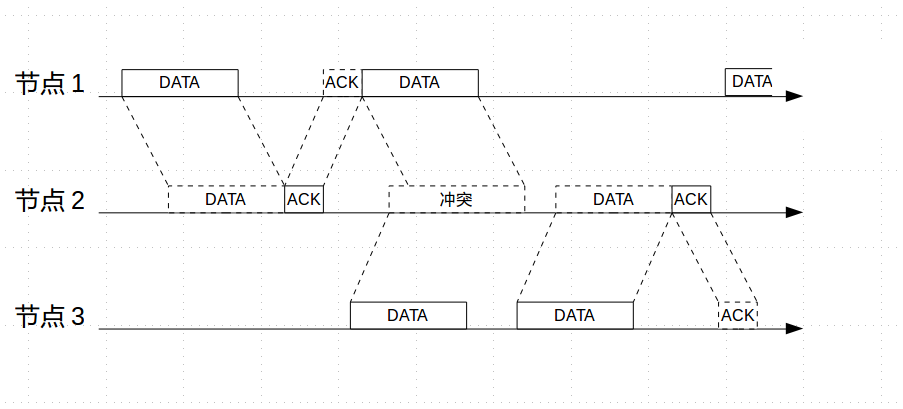
\includegraphics[scale=0.4]{figures/aloha.png}
	\caption{
		移动节点接入离开机制
	}
	\label{fig:example}
\end{figure}

\subsection{性能分析}
\cite{Analysis of Aloha Protocols for Underwater Acoustic Sensor Networks}
UWALHOHA协议数据发送成功指的是在t时刻,有且只有一个节点发送的数据到达,并且没有与其他数据产生碰撞的场景。这意味着如果一个数据要经过$\Delta t$时间传播,那么它不可以在$t-\Delta t$时间发送。

假设节点在t时刻发送数据的概率为$p$,其他$n-1$个节点不发送数据的概率为$p-1$,信道传输的成功概率为:
\begin{equation}
P_S=p(1-p)^{n-1}   0\le p\le 1
\end{equation}
最优传输成功率为:
\begin{equation}
\lim\limits_{n\to+\infty} (1-\frac{1}{n})^{n-1}=\frac{1}{e}
\end{equation}
\section{SFAMA}

\subsection{原理}
当一个节点想要进行一次数据交互时,它会等待到下一个时隙时间开始传送RTS帧。目标节点和其他邻居节点会在当前时隙内接收到RTS帧。目标节点在下一个时隙开始时发送CTS帧,CTS帧会被源节点和目标节点的邻居节点接收到。源节点接收到CTS帧后,在下一个时隙时间传送DATA帧,其他邻居节点接收到CTS帧后进行退避。目标节点接收到全部数据后在下一个时隙时间发送ACK帧确认。

\begin{figure}[ht]
	\centering
	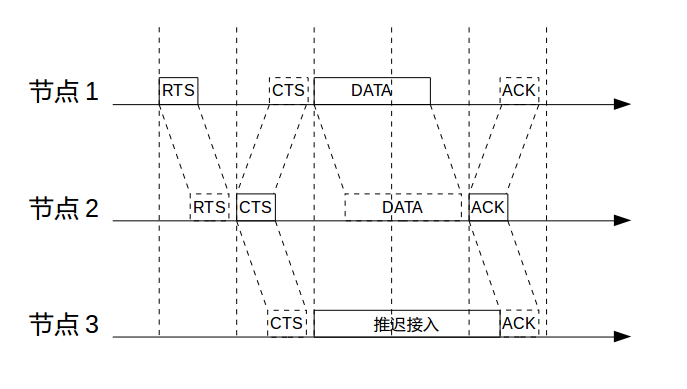
\includegraphics[scale=0.4]{figures/sf.png}
	\caption{
		移动节点接入离开机制
	}
	\label{fig:example}
\end{figure}

\subsection{性能分析}
假设$P_S$是信道传输的成功(无碰撞)概率。无碰撞概率指的是在节点$\omega$传输的时间间隙内没有邻居节点进行传输的概率。邻居节点可能会传输RTS帧或者还没有被接收的CTS帧进而引起碰撞。例如节点$\alpha$是节点$\omega$和节点$\beta$的邻居节点,节点$\beta$是节点$\omega$的隐藏终端。节点$\alpha$在第$n-1$时隙内向节点$\beta$发送了RTS帧,节点$\omega$在第$n$时隙内向节点$\alpha$发送了RTS帧,那么节点$\omega$的RTS帧和节点$\alpha$要发送的CTS帧会在第n时隙产生冲突。

对于节点$\omega$的任一邻居节点,隐藏终端数量假设为Q。任一隐藏终端以$\lambda/N$的速率向节点$\omega$的邻居节点发送RTS包,信道传输的成功概率为:
\begin{equation}
\begin{aligned}
P_S=\prod^N_1 e^{-\lambda T_{slot}}\cdot \prod^N_1 (\prod^Q_1 e^{-\frac{\lambda}{N} T_{slot}})= e^{-\lambda (N+Q) T_{slot}}
\end{aligned}
\end{equation}

一个失败周期的持续时间是两个时隙长度,第一个时隙发送RTS,第二个时隙等待接收CTS超时。所有N+1个节点以相同速率传递RTS,节点$\omega$传输RTS的速率是$\frac{1}{N+1}$,所以
\begin{equation}
\overline T_{fail}=\frac{{2T_{slot}}\cdot(1-P_S)}{N+1}
\end{equation}

一个成功周期的持续时间包括了RTS,CTS,DATA(包括由误码引起的重传时间)和ACK传输时间。假设$T_{data}$是一个DATA包传输所需要的全部时间,$T_{tot}$是一个成功周期持续时间,
\begin{equation}
T_{tot}=3T_{slot}+T_{data}
\end{equation}
\begin{equation}
\overline T_{success}=P_S \cdot T_{tot}
\end{equation}

节点的推迟接入时间包括了侦听到其他节点的CTS帧后的推迟时间和侦听到信道冲突后的推迟时间两部分,
\begin{equation}
\overline T_{defer}=(T_{data}+T_{slot})(\frac{QP_S}{N+1}+\frac{N}{N+1}(1-P_S)) 
\end{equation}

信道平均空闲时间为:
\begin{equation}
\overline I=\frac{1}{(N+1)\lambda}
\end{equation}

假设数据传输时间为$\delta$,则平均数据传输时间为
\begin{equation}
\overline U=\frac{\delta}{(N+1)P_S}
\end{equation}

根据吞吐量公式,计算得单一节点的吞吐量$(S)$为
\begin{equation}
\begin{aligned}
S&=\frac{\overline U}{\overline B+\overline I}=\frac{\overline U}{\overline T_{success}+\overline T_{fail}+\overline T_{defer}+\overline I}\\
&=\frac{\delta P_s}{(n+1)P_S T{tot}+2T_{slot}+(T_{data}+T_{slot})(QP_S+N(1-P_S))+\frac{1}{\lambda}}
\end{aligned}
\end{equation}

\endinput